
Lean UX \citep{Gothelf2013} es el enfoque o metodología que acompaña la construcción del prototipo de este trabajo final, a continuación se explican los conceptos que motivan la elección de esta metodología.


Desde 1980 hasta fines de 1990 los diseñadores se enfocaron en el diseño de software de la misma manera que lo habían hecho con el resto de los materiales. \vskip
Cuando se diseña para producir un objeto tangible, se necesita tener muy claro lo que se hace antes de iniciar la producción física, porque la producción es costosa, es costoso poner en marcha una fábrica para producir bienes físicos. \vskip En el ámbito del desarrollo de software, los diseñadores tuvieron que enfrentar nuevos retos, descubrir los nuevos medios y, a medida que lo hacían, aparecían nuevas especialidades, como el diseño de interacción o la arquitectura de información. Sin embargo, en esa época la práctica de los diseñadores apenas cambió. Todavía diseñaban los productos de manera tradicional, con mucho detalle y por adelantado, porque había un proceso de ``fabricación": había que hacer copias de los trabajo en discos flexibles y CDs y distribuirlas de la misma manera en la que se distribuyen los bienes físicos. Cometer errores en ese contexto se traducía en enormes costos de producción. \vskip

Internet cambió la lógica de distribución de software de una manera radical, la mayoría del software hoy en día se distribuye en línea y al desaparecer el proceso físico de fabricación se puede trabajar con ciclos de producción mucho más cortos.
Los equipos de desarrollo de software utilizan técnicas como el desarrollo ágil, la integración continua y el despliegue continuo reduciendo drásticamente el tiempo para generar nuevas cambios en el software. Estos equipos realizan cambios en el código y suben los cambios a producción\footnote{Producción es la instancia del software a disposición de los usuarios finales.} con velocidad similar a la acción de guardar cualquier archivo en una computadora. Además, utilizan esos ciclos cortos como ventaja competitiva, producen nuevas versiones del software en tiempos acotados, lo que permite obtener retroalimentación del mercado e iterar incorporando lo que han aprendido y tal vez sin advertirlo aumentan las expectativas de los clientes que pueden obtener más calidad en menos tiempo. En este nuevo contexto, las prácticas de pensar todo al inicio de los procesos quedaron obsoletas. \vskip
\textit{Lean User Experience} (Lean UX) se puede traducir como \textit{Experiencia de Usuario limpia o sin desperdicios} y se describe como una nueva etapa evolutiva en el diseño de productos. Su objetivo es tomar las mejores herramientas del diseño y adaptarlas a esta nueva realidad.

Lean UX es profundamente colaborativo, en gran medida porque:
\begin{itemize}

    \item Logra que los diseñadores no están aislados del resto del equipo de trabajo.
    \item Permite implementar técnicas para construir una comprensión compartida del proyecto. 
    \item Logra un clima propicio para la retroalimentación con los usuarios finales y  replantea las conversaciones de diseño en términos objetivos, se pueden obtener métricas sobre las funcionalidades, analizar y ajustar.
    \item Cambia la forma en que se comunica el diseño del producto: en lugar de comunicar características y documentos exhaustivos se puede comunicar funcionalidad.
\end{itemize}

 
\vskip


Los 3 pilares principales de Lean UX son:
\begin{enumerate}
    \item \textbf{Design Thinking o Pensamiento de Diseño:} Alienta al equipo a colaborar en todas las etapas del proyecto y a considerar el producto desde una perspectiva global, utilizando la sensibilidad y los métodos de los diseñadores para satisfacer las necesidades del usuario final con soluciones tecnológicamente viables.

    \item \textbf{Desarrollo Ágil}:
     Aplica los cuatro principios básicos del desarrollo Ágil al diseño de los productos.
        
\begin{itemize}
\item
\textbf{Los individuos y las interacciones son más importantes que los procesos y las herramientas}\vskip
Para generar rápidamente las mejores soluciones, es necesario implicar al todo el equipo. El intercambio de ideas deberá ser libre y frecuente. La conversación fluida entre colegas deberá primar por encima de las restricciones propias de las herramientas, ya sea en los procesos o en la producción.
\item
\textbf{El software funcional es más importante que la documentación exhaustiva}\vskip
Se pueden encontrar múltiples soluciones para todos los problemas de negocio y todos los miembros del equipo podrán tener una opinión diferente de cuál es la mejor. El reto está en averiguar cuál de ellas es la que tiene más posibilidades. Por eso, cuanto antes se cuente con un software que funcione, antes se puede encontrar la solución que mejor se adapte a los requerimientos.
\item
\textbf{La colaboración con los clientes es más importante que la negociación de contratos con ellos}\vskip
Si el equipo colabora con los usuarios/clientes, hay un entendimiento común sobre los problemas y las posibles soluciones. Cualquier decisión que se adopte después se tomará por consenso, lo que se traduce en iteraciones más rápidas y una verdadera implicación de todos los actores con la ventaja de trabajar siempre con soluciones validadas. Además, como todos los miembros del equipo participan en la toma de decisiones, no se requieren tantas entregas de documentación por escrito.
\item
\textbf{La respuesta a los cambios es más importante que la planificación}\vskip
Lean UX asume que los diseñadores del producto inicial no encontrarán la solución a la primera, por lo que el objetivo consiste en averiguar qué han hecho mal lo antes posible. Una vez que se descubra lo que funciona y lo que no, se pueden ajustar las propuestas y volver a probarlas. Así, la retroalimentación mantendrá ágil al equipo, dirigiendo la solución siempre en la dirección correcta.
\end{itemize}

\item \textbf{Método Lean Startup}: Utiliza un bucle de retroalimentación llamado  ``Construir-Medir-Aprender" para minimizar el riesgo del proyecto, haciendo que los equipos construyan y aprendan rápidamente.
Los equipos construyen productos viables mínimos en inglés \textit{Minimum Viable Product} (MVP) y los envían para comenzar el proceso de aprendizaje tan pronto como sea posible.\vskip
Lean Startup\footnote{\url{https://es.wikipedia.org/wiki/Lean_startup} }  desde el principio aboga por la creación de prototipos rápidos para comprobar, por un lado, que las suposiciones son correctas y, por otro, para conseguir retroalimentación de los usuarios de forma inmediata y así poder mejorar el software más rápido que las prácticas tradicionales de ingeniería de software.\vskip
Lean UX, por su parte, es una implementación directa de esta filosofía aplicada al diseño de productos. Cada diseño es una solución propuesta, una hipótesis. Su objetivo consiste en validar la solución de la manera más eficiente posible mediante la realimentación. El componente más pequeño que se puede construir para probar cada hipótesis es el Producto Viable Mínimo MVP. 

\begin{figure}[h]
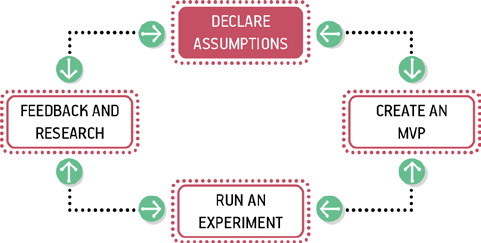
\includegraphics[width=10cm]{Img/UX/UX-0.png}
\centering
\caption{\textbf{ \footnotesize{Enfoque LEAN UX. }}}
\end{figure}
\end{enumerate}

Lean UX funciona como una práctica para entender rápidamente la función de un producto. Para ello elije un camino colaborativo y multidisciplinario; reduce el énfasis por la documentación exhaustiva y aumenta el enfoque en la construcción de un entendimiento compartido del producto que está siendo diseñado. Como consecuencia de usar este enfoque se obtiene: un equipo que trabaja de forma colaborativa, iterativamente, reduciendo al mínimo los documentos entregables, enfocándose en el software funcional y en la retroalimentación con el usuario final.

Por todo lo señalado se considera que este enfoque es el adecuado para abordar el trabajo en la aplicación COCADA. Las etapas de LEAN UX se pueden ver aplicadas en este documento en el capítulo \ref{chap: cap3} correspondiente al desarrollo del prototipo.



Agregar lo de chaos report http://www.laboratorioti.com/2016/05/16/informe-del-caos-2015-chaos-report-2015-bien-mal-fueron-los-proyectos-ano-2015/

https://modelometodoygestion.wordpress.com/2017/02/21/chaos-report-15-scrum/

Ver frase final para chamu
http://www.uxline.com/blog/agile-ux-versus-lean-ux/



VER LO DE FUZZY DESIGN y agregar tambien a la parte de codiseño

https://blog.prototypr.io/the-teapot-model-how-to-explain-a-fuzzy-design-process-to-anxious-clients-4a2e8487bc87


COMO ENGANCHAR TODO
https://es.linkedin.com/pulse/design-thinking-lean-startup-agile-victor-mansilla


https://www.cio.com/article/3174516/project-management/it-project-success-rates-finally-improving.html



https://www.pmi.org/-/media/pmi/documents/public/pdf/learning/thought-leadership/pulse/pulse-of-the-profession-2017.pdf